% Options for packages loaded elsewhere
\PassOptionsToPackage{unicode}{hyperref}
\PassOptionsToPackage{hyphens}{url}
%
\documentclass[
  10pt,
]{article}
\usepackage{amsmath,amssymb}
\usepackage{iftex}
\ifPDFTeX
  \usepackage[T1]{fontenc}
  \usepackage[utf8]{inputenc}
  \usepackage{textcomp} % provide euro and other symbols
\else % if luatex or xetex
  \usepackage{unicode-math} % this also loads fontspec
  \defaultfontfeatures{Scale=MatchLowercase}
  \defaultfontfeatures[\rmfamily]{Ligatures=TeX,Scale=1}
\fi
\usepackage{lmodern}
\ifPDFTeX\else
  % xetex/luatex font selection
\fi
% Use upquote if available, for straight quotes in verbatim environments
\IfFileExists{upquote.sty}{\usepackage{upquote}}{}
\IfFileExists{microtype.sty}{% use microtype if available
  \usepackage[]{microtype}
  \UseMicrotypeSet[protrusion]{basicmath} % disable protrusion for tt fonts
}{}
\makeatletter
\@ifundefined{KOMAClassName}{% if non-KOMA class
  \IfFileExists{parskip.sty}{%
    \usepackage{parskip}
  }{% else
    \setlength{\parindent}{0pt}
    \setlength{\parskip}{6pt plus 2pt minus 1pt}}
}{% if KOMA class
  \KOMAoptions{parskip=half}}
\makeatother
\usepackage{xcolor}
\usepackage[margin=0.7in]{geometry}
\usepackage{longtable,booktabs,array}
\usepackage{calc} % for calculating minipage widths
% Correct order of tables after \paragraph or \subparagraph
\usepackage{etoolbox}
\makeatletter
\patchcmd\longtable{\par}{\if@noskipsec\mbox{}\fi\par}{}{}
\makeatother
% Allow footnotes in longtable head/foot
\IfFileExists{footnotehyper.sty}{\usepackage{footnotehyper}}{\usepackage{footnote}}
\makesavenoteenv{longtable}
\usepackage{graphicx}
\makeatletter
\def\maxwidth{\ifdim\Gin@nat@width>\linewidth\linewidth\else\Gin@nat@width\fi}
\def\maxheight{\ifdim\Gin@nat@height>\textheight\textheight\else\Gin@nat@height\fi}
\makeatother
% Scale images if necessary, so that they will not overflow the page
% margins by default, and it is still possible to overwrite the defaults
% using explicit options in \includegraphics[width, height, ...]{}
\setkeys{Gin}{width=\maxwidth,height=\maxheight,keepaspectratio}
% Set default figure placement to htbp
\makeatletter
\def\fps@figure{htbp}
\makeatother
\setlength{\emergencystretch}{3em} % prevent overfull lines
\providecommand{\tightlist}{%
  \setlength{\itemsep}{0pt}\setlength{\parskip}{0pt}}
\setcounter{secnumdepth}{-\maxdimen} % remove section numbering
\ifLuaTeX
  \usepackage{selnolig}  % disable illegal ligatures
\fi
\usepackage{bookmark}
\IfFileExists{xurl.sty}{\usepackage{xurl}}{} % add URL line breaks if available
\urlstyle{same}
\hypersetup{
  hidelinks,
  pdfcreator={LaTeX via pandoc}}

\author{}
\date{}

\begin{document}

\section{Deterministic coefficient descent on rational-point
bases}\label{deterministic-coefficient-descent-on-rational-point-bases}

2026-11-14. Source \texttt{1e3f20752022a341a4612e6a72e8e5690f8c6baa}.
All claims unsigned {[}pcc:unverified{]}.

For a factor base made of actual prime-field points, every successful
bounded monic norm pair in the stated model has prime-field
coefficients, even when initially sought over an extension field. The
proof derives its successful support and branch signs from the
norm/divisibility equations. It does not receive them as oracles. The
abstract pole-window result has arbitrary arity; the existing
four-coefficient chart has a separate exact membership corollary
{[}pcc:unverified{]}.

Central claims: support selection \texttt{PCC-20261114-20a4bc}, general
rigidity \texttt{PCC-20261114-8c21e7}, prime coefficients
\texttt{PCC-20261114-255fa5}, actual norm divisor
\texttt{PCC-20261114-0943a7}, actual core \texttt{PCC-20261114-5d35b3}.
\href{../lean/NormSplitBaseDescent.lean}{Lean source},
\href{../SPLIT_BASE_DESCENT_PROTOCOL.md}{prospective contract},
\href{../split-base-descent-evidence/claim-pins.json}{exact proof map},
\href{descent.dot}{editable diagram}, \href{descent.svg}{SVG},
\href{report.pdf}{PDF}.

\begin{figure}
\centering
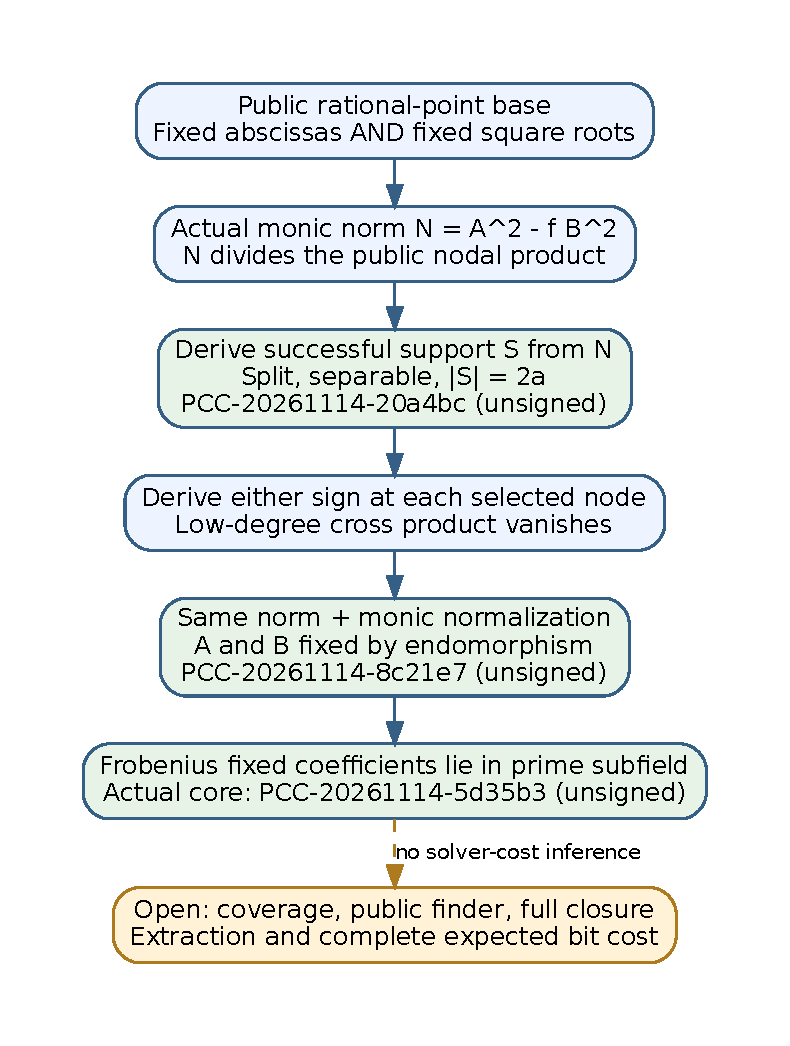
\includegraphics[width=0.85\textwidth,height=\textheight]{descent.pdf}
\caption{Successful support and signs are consequences of actual norm
divisibility on a public rational-point base. Frobenius rigidity then
gives prime-field coefficients. No finder or cost bound follows.
Evidence unsigned.}
\end{figure}

\subsection{Exact general statement}\label{exact-general-statement}

Let \(L\) be a field of characteristic a prime \(p\). Let \(T\subset L\)
be a finite set of distinct public abscissas, all in the prime subfield.
Let \(f\in L[X]\) have degree at most3 and prime-subfield coefficients.
For every \(x\in T\), require a public prime-subfield square root of
\(f(x)\). Thus these are actual rational curve points, rather than
arbitrary rational abscissas that may lift only on a twist
{[}pcc:unverified{]}.

Suppose a candidate has

\[
A\text{ monic},\quad \deg A=a,\quad \deg B<a-1,\quad
N=A^2-fB^2\mid P_T=\prod_{x\in T}(X-x).
\]

Then every coefficient of \(A\) and \(B\) belongs to the prime subfield.
The proof establishes that \(N\) is monic of degree \(2a\). The source
uses natural degrees, whose lower-polynomial guard implies \(a\ge2\).
Zero \(B\) is not silently excluded. The hypotheses are actual
certificate equations and degree guards; no public finder algorithm,
favorable closure bound or efficient support-selection assumption
appears {[}pcc:unverified{]}.

This statement is algebraic. Applying its certificates to an elliptic
group/scalar relation still uses the existing group bridge and its
nonsingularity, distinct-point and label premises. The theorem itself
does not manufacture those scalar labels {[}pcc:unverified{]}.

\subsection{Why the support and signs need not be
supplied}\label{why-the-support-and-signs-need-not-be-supplied}

Since \(P_T\) splits and has distinct roots, its monic divisor \(N\)
splits and is separable. The proof takes the roots of \(N\) as a finite
set \(S\), derives \(S\subseteq T\), and proves {[}pcc:unverified{]}

\[N=\prod_{x\in S}(X-x),\qquad |S|=2a.\]

This is a mathematical derivation from divisibility, not an efficient
method for finding the unknown divisor \(N\) {[}pcc:unverified{]}.

Let \(\phi\) be a field endomorphism fixing the public abscissas, public
square roots and curve coefficients. At a selected node, the norm gives
\(A(x)^2=y^2B(x)^2\). Factoring the difference of squares derives either
sign. Because \(y\) is fixed, either case gives

\[A(x)\phi(B(x))-\phi(A(x))B(x)=0.\]

No nonzero \(B(x)\) or successful sign is assumed. Write
\(A^\phi,B^\phi\) for coefficientwise images. The cross polynomial
\(AB^\phi-A^\phi B\) therefore vanishes on \(S\) and has degree below
\(2a\); it is zero. Mapping the actual norm preserves \(N\). Equal norms
and zero cross product give proportional square polynomials. Monic upper
normalization forces the scalar to1, hence

\[A^\phi=A,\qquad B^\phi=B.\]

The lower polynomial may be zero. This is why neither a division by its
value nor a discarded exceptional case is needed {[}pcc:unverified{]}.

With \(\phi\) equal to Frobenius, every coefficient \(c\) satisfies
\(c^p=c\). Mathlib's exact prime-subfield fixed-point theorem gives
\(c\in\mathbf F_p\). A separate theorem provides literal polynomial
lifts to the prime subfield. No agreement-on-sampled-values argument is
used {[}pcc:unverified{]}.

\subsection{Binding to the existing actual
chart}\label{binding-to-the-existing-actual-chart}

For the current chart, retain the exact target completion

\[
D=X^3+a_2X^2+a_1X,\quad B=c_0+c_1X,\quad
A=D+zB(r)-D(r),\quad z^2=r^3+ar+b.
\]

Let the public target abscissa \(r\) lie outside the rational base
\(T\), and compute the actual monic support

\[U=(A^2-fB^2)\operatorname{div}(X-r).\]

The input equation is the actual remainder \(P_T\bmod U=0\). Its monic
division guard yields \(U\mid P_T\), hence the full actual norm divides
\((X-r)P_T=P_{T\cup\{r\}}\). Target coordinates and every allowed base
point are prime-field data. The general result now forces
\(a_1,a_2,c_0,c_1\) into the prime subfield. The source proves the upper
and lower degree guards and extracts these actual polynomial
coefficients {[}pcc:unverified{]}.

This corollary is the fixed monic degree5 support chart. The abstract
rigidity theorem is not restricted to it. Neither statement is a
growing-family solver-complexity theorem, nor a claim about arbitrarily
redundant free slack variables {[}pcc:unverified{]}.

\subsection{The factor-base change and its cost
obligation}\label{the-factor-base-change-and-its-cost-obligation}

The base premise is changed openly. It is not a transfer of the earlier
Kummer rationality result to Dickson fibers or arbitrary input primes.
The following comparison records theorem scope, not measured performance
{[}pcc:unverified{]}.

\begin{longtable}[]{@{}
  >{\raggedright\arraybackslash}p{(\columnwidth - 4\tabcolsep) * \real{0.3333}}
  >{\raggedright\arraybackslash}p{(\columnwidth - 4\tabcolsep) * \real{0.3333}}
  >{\raggedright\arraybackslash}p{(\columnwidth - 4\tabcolsep) * \real{0.3333}}@{}}
\toprule\noalign{}
\begin{minipage}[b]{\linewidth}\raggedright
Item
\end{minipage} & \begin{minipage}[b]{\linewidth}\raggedright
Earlier Kummer review
\end{minipage} & \begin{minipage}[b]{\linewidth}\raggedright
Current rational-point base
\end{minipage} \\
\midrule\noalign{}
\endhead
\bottomrule\noalign{}
\endlastfoot
Allowed abscissas & A Kummer coset; rational lifts may fail & Explicit
actual rational points \\
Rationality mechanism & Good-coset and short mixed-twist relation
exclusions & Deterministic norm/Frobenius rigidity \\
Field conditions for that implication & Includes an admissible 2-power
divisor of \(p-1\) and other stated premises & Prime characteristic and
the explicit rational-point premises \\
Membership representation & Structured tower & Public nodal product of
degree \(|T|\); no cheap tower assumed \\
Finder and complete cost & Unresolved & Unresolved \\
\end{longtable}

Known scalar multiples of the input generator are a prospective way to
obtain actual rational base points with labels in a fresh attempt. This
is not a novel generator claim or free reusable precomputation. Base
construction, duplicate/opposite/target exclusions, membership encoding,
coverage, failed attempts and solver work must all be charged. No such
coverage or cost bound is established by this component
{[}pcc:unverified{]}.

The next central obligation remains a constructive public finder with
bounded growing-family normal forms or closure. This descent result
removes the mixed-twist field-of-definition issue for this base; it does
not turn an algebraic-closure solver into an efficient algorithm or
bound its extraction work {[}pcc:unverified{]}.

\subsection{Sources, validation and retained
failures}\label{sources-validation-and-retained-failures}

Sources checked (KB): unavailable as already recorded, no unchanged
retry. The
\href{../split-base-descent-evidence/prior-search-receipt.json}{bounded
receipt} records actual source paths and query scope. Read the
independent Kummer
\href{https://github.com/isogeny-labs/crypto/blob/f87e25bb0b50a5ce137eaa33fc733d317a2f0981/research/prime_one_shot_20261029/continuation/reviews/rationality.md}{rationality
review}, the actual norm uniqueness sources, and pinned Mathlib
split/separable, nodal and prime-subfield declarations. Earlier
elliptic-code and non-Semaev reports remain scoped to their received
words and generic-target-access assumptions. These standard ingredients
and bounded searches establish no novel algorithm or exhaustive absence
{[}pcc:unverified{]}.

Final module build007 exits0 with no warnings and14 authored statements;
only standard foundations are printed. The whole-study gate audits383
statements with0 additional trusted uses, exit0. Import-inclusive fresh
replay exits0. Validation receipt PCC-20261114-7b5216 pins source and
raw logs in
\href{../split-base-descent-evidence/validation-001.json}{validation-001.json}.
All15 claims are unsigned/default not\_covered, exit2
{[}pcc:unverified{]}.

All failed drafts001 through006 remain. They record protected-map and
identity-wrapper errors, a redundant tactic, an explicit characteristic
parameter, finite-set equality instance, constant-power simplification
and an omitted existing call argument. No statement was weakened, check
suppressed or trusted axiom added. No Rust/native source changed and no
prior native tests are counted again {[}pcc:unverified{]}.

No fixture, unknown-root, F4/msolve, paid/cloud/attack or timing
experiment was launched. The earlier native fixture remains1 planned,0
attempted, 0 completed,0 excluded,1 admission-blocked by unchanged
checkpoint upload transport. Local universal proof construction is
separate. Global performance/curve/attack-route graphs stay unchanged:
no measured speedup or new group-transport edge is claimed
{[}pcc:unverified{]}.

\subsection{Exact proof map}\label{exact-proof-map}

All bindings unsigned {[}pcc:unverified{]}. Exact declarations/context
hashes and source freeze are retained in claim-pins.json.

\begin{longtable}[]{@{}ll@{}}
\toprule\noalign{}
Declaration & Claim \\
\midrule\noalign{}
\endhead
\bottomrule\noalign{}
\endlastfoot
\texttt{branchCross} & \texttt{PCC-20261114-51b429} \\
\texttt{evalMapFixed} & \texttt{PCC-20261114-955ed2} \\
\texttt{nodalMapFixed} & \texttt{PCC-20261114-e742aa} \\
\texttt{crossFromNorm} & \texttt{PCC-20261114-a916b6} \\
\texttt{monicPairUnique} & \texttt{PCC-20261114-401e74} \\
\texttt{pairFixedOnNodes} & \texttt{PCC-20261114-3d0e01} \\
\texttt{divisorSupport} & \texttt{PCC-20261114-20a4bc} \\
\texttt{normWindow} & \texttt{PCC-20261114-1f4820} \\
\texttt{pairFixedFromDivisor} & \texttt{PCC-20261114-8c21e7} \\
\texttt{frobeniusFixedIff} & \texttt{PCC-20261114-68c109} \\
\texttt{pairPrimeCoefficients} & \texttt{PCC-20261114-255fa5} \\
\texttt{primePolynomialLift} & \texttt{PCC-20261114-bde010} \\
\texttt{actualNormDivides} & \texttt{PCC-20261114-0943a7} \\
\texttt{actualCorePrimeCoefficients} & \texttt{PCC-20261114-5d35b3} \\
\end{longtable}

\end{document}
